\documentclass[a4paper]{article}
\usepackage[utf8]{inputenc}
\usepackage[ngerman]{babel}
\usepackage{listings}
\usepackage{float}
\usepackage{graphicx}
\usepackage{color}
\usepackage{listings}
\usepackage[dvipsnames]{xcolor}
\usepackage{tabularx}
\usepackage{geometry}
\usepackage{color,graphicx,overpic}
\usepackage{amsmath,amsthm,amsfonts,amssymb}
\usepackage{tabularx}
\usepackage{listings}
\usepackage[many]{tcolorbox}
\usepackage{multicol}

\newtheorem{definition}{Definition}
\newtheorem{proposition}{Proposition}
\newtheorem{beweis}{Beweis}

\pdfinfo{
    /Title (Automaten, Sprachen \& Komplexität - Übung)
    /Creator (TeX)
    /Producer (pdfTeX 1.40.0)
    /Author (Robert Jeutter)
    /Subject ()
}

% Don't print section numbers
\setcounter{secnumdepth}{0}

%My Environments
\newtheorem{example}[section]{Example}


\newtcolorbox{myboxii}[1][]{
  breakable,
  freelance,
  title=#1,
  colback=white,
  colbacktitle=white,
  coltitle=black,
  fonttitle=\bfseries,
  bottomrule=0pt,
  boxrule=0pt,
  colframe=white,
  overlay unbroken and first={
  \draw[red!75!black,line width=3pt]
    ([xshift=5pt]frame.north west) -- 
    (frame.north west) -- 
    (frame.south west);
  \draw[red!75!black,line width=3pt]
    ([xshift=-5pt]frame.north east) -- 
    (frame.north east) -- 
    (frame.south east);
  },
  overlay unbroken app={
  \draw[red!75!black,line width=3pt,line cap=rect]
    (frame.south west) -- 
    ([xshift=5pt]frame.south west);
  \draw[red!75!black,line width=3pt,line cap=rect]
    (frame.south east) -- 
    ([xshift=-5pt]frame.south east);
  },
  overlay middle and last={
  \draw[red!75!black,line width=3pt]
    (frame.north west) -- 
    (frame.south west);
  \draw[red!75!black,line width=3pt]
    (frame.north east) -- 
    (frame.south east);
  },
  overlay last app={
  \draw[red!75!black,line width=3pt,line cap=rect]
    (frame.south west) --
    ([xshift=5pt]frame.south west);
  \draw[red!75!black,line width=3pt,line cap=rect]
    (frame.south east) --
    ([xshift=-5pt]frame.south east);
  },
}

\begin{document}
\begin{myboxii}[Disclaimer]
    Die Übungen die hier gezeigt werden stammen aus der Vorlesung \textit{Algorithmen, Sprachen und Komplexität}! Für die Richtigkeit der Lösungen wird keine Gewähr gegeben.
\end{myboxii}


%%%%%%%%%%%%%%%%%%%%%%%%%%%%%%%%%%%%%%%%%%%%%%%%%%%%%%%%%%%%%%%%%%%%%%%%%%%%%%%%%%%%%%%%%%%%%%%%%%%%%%%%%%%%%%%%%%%%
\section{Übung 00}
%##########################################
\subsection{Aufgabe 1}
\textit{Das Schubfachprinzip besagt: Wenn $n$ Objekte auf $m$ Schubladen verteilt werden mit $n > m > 0$, dann gibt es eine Schublade, die mindestens zwei Objekte enthält.}
\textit{Zeigen Sie, dass es mindestens zwei Personen in Deutschland mit gleich vielen Haaren gibt.}

\textit{(b) Beweisen Sie das verschärfte Schubfachprinzip: Verteilt man n Objekte auf m Schubladen mit $n > m > 0$, dann gibt es eine Schublade, die mindestens $\lceil \frac{n}{m}\rceil$ Objekte enthält}

%##########################################
\subsection{Aufgabe 2}
\textit{Zeigen Sie per vollständiger Induktion über $n\geq 0$, dass es in jedem Binärbaum mit mindestens $2^n$ Blättern einen Pfad der Länge mindestens $n$ von der Wurzel zu einem Blatt gibt.}

%##########################################
\subsection{Aufgabe 3}
\textit{Eine Menge A heißt gleichmächtig zu einer Menge B, wenn es eine Bijektion von A nach B gibt. Zeigen Sie:}

\textit{(a) Die Menge der natürlichen Zahlen $\mathbb{N}$ ist nicht gleichmächtig zur Menge der reellen Zahlen $\mathbb{R}$.}

\textit{(b) Keine Menge ist gleichmächtig zu ihrer Potenzmenge. (Satz von Cantor)}

\newpage
%%%%%%%%%%%%%%%%%%%%%%%%%%%%%%%%%%%%%%%%%%%%%%%%%%%%%%%%%%%%%%%%%%%%%%%%%%%%%%%%%%%%%%%%%%%%%%%%%%%%%%%%%%%%%%%%%%%%
\section{Übung 01}
%##########################################
\subsection{Aufgabe 1}
\textit{Es sind die DFAs $M_1$ und $M_2$ und die NFAs $M_3$ und $M_4$ (von links nach rechts) gegeben.}
\begin{center}
    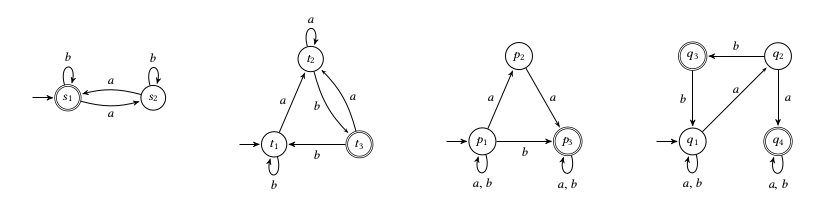
\includegraphics[width=1\linewidth]{Assets/ASK_uebung/u01-01.png}
\end{center}
\textit{Bearbeiten Sie die folgenden Teilaufgaben für alle $i\in \{1, 2, 3, 4\}$.}

\textit{(a) Geben Sie jeweils zwei Wörter an, die von $M_i$ akzeptiert bzw. nicht akzeptiert werden.}

\textit{(b) Geben Sie analog zu Aufgabe 2 eine kurze aber präzise Beschreibung der Sprache $L(M_i)$ an.}


%##########################################
\subsection{Aufgabe 2}
\textit{Betrachten Sie die nachfolgenden Sprachen über dem Alphabet $\sum = \{a, b\}$.
    \begin{itemize}
        \item $L_1 = \{w \in\sum^* \vert \text{w enthält die Zeichenfolge baba}\}$
        \item $L_2 = \sum^* \backslash \{aa, ab, aab\}$
        \item $L_3 = \{w \in\sum^* \vert \text{es existiert } k \geq 1 \text{, so dass w mit } a(ab)^k \text{ beginnt}\}$
        \item $L_4 = \{w\in\sum^* \vert \text{w endet auf aab}\}$
    \end{itemize}
    Geben Sie für alle $i\in\{1, 2, 3, 4\}$ jeweils einen DFA $M_i$ mit $L(M_i)=L_i$ grafisch an. Wählen Sie jeweils zwei Wörter aus $L_i$ und $\sum^*\backslash L_i$ aus und überprüfen Sie, ob $M_i$ auf diesen korrekt arbeitet.}

%##########################################
\subsection{Aufgabe 3}
\textit{Konstruieren Sie mit der Potenzmengenkonstruktion einen DFA, der die gleiche Sprache akzeptiert, wie $M_3$ aus Aufgabe 1.}

%##########################################
\subsection{Aufgabe 4}
\textit{Sei $\sum = \{a, b, c\}$. Unter den folgenden 16 Sprachen über $\sum$ befinden sich acht Paare gleicher Sprachen. Finden Sie heraus, welche Sprachen gleich sind und begründen Sie jeweils in maximal zwei Sätzen, warum die entsprechende Gleichheit gilt.}
\begin{multicols}{2}
    $$L_1 = \{w \in \sum^* \vert \quad\vert w\vert_a = \vert w\vert_b = \vert w\vert_c \}$$
    $$L_2 = \{w \in \sum^* \vert \quad\vert w\vert_a = \vert w\vert_b \}$$
    $$L_3 = \{w \in \sum^* \vert \quad\vert w\vert_a = 0\}$$
    $$L_4 = \{w \in \sum^* \vert \quad\vert w\vert_a = 2\}$$
    $$L_5 = \{w \in \sum^* \vert \quad\vert w\vert_a = 4\}$$
    $$L_6 = \{b, c\}^*\{a\}\{b, c\}^* \{a\}\{b, c\}^*$$
    $$L_7 = \{a\}\{ba\}^*\{b\}$$
    $$L_8 = \{a^n b^n \vert n \in \mathbb{N}\}$$
    $$L_9 = L_2 \cap \{a\}^*\{b\}^*$$
    $$L_{10} = L_2 \cap \{w \in \sum^* \vert \quad\vert w \vert_b = \vert w\vert_c\}$$
    $$L_{11} = (L_3 L_4 )^2$$
    $$L_{12} = \sum^* \backslash L_3$$
    $$L_{13} = L_2^3$$
    $$L_{14} = \{ab\}^+$$
    $$L_{15} = \{b, c\}^*$$
    $$L_{16} = \sum^* \{a\}\sum^*$$
\end{multicols}

%##########################################
\subsection{Aufgabe 5}
\textit{Sei $\sum=\{a, b\}$. Für $n\in\mathbb{N}$ sei $\sum^{\leq n} = \bigcup_{i\leq n} \sum^i$ die Menge der Wörter in $\sum$ deren Länge höchstens $n$ ist. Zeigen Sie per vollständiger Induktion über $n\in\mathbb{N}$, dass $\vert\sum^{\leq n}\vert = 2^{n+1} - 1$.}

%##########################################
\subsection{Aufgabe 6}
\textit{Gegeben sei die Grammatik $G = (\{S, A, B, C\}, \{a, b, c\}, P, S)$, wobei P genau die folgenden Produktionen enthält:
    \begin{multicols}{3}
        $$S\rightarrow A \vert C$$
        $$A \rightarrow Aa \vert a$$
        $$Bb \rightarrow bb$$
        $$Bc \rightarrow bbc$$
        $$C \rightarrow BCc \vert c.$$
    \end{multicols}
}

\textit{(a) Geben Sie eine Ableitung von bbbccc an.}

\textit{(b) Geben Sie eine möglichst kurze aber präzise Beschreibung von L(G) an. Begründen Sie Ihre Antwort.}

%##########################################
\subsection{Aufgabe 7}
\textit{Konstruieren Sie Grammatiken $G_1, G_2$ und $G_3$ so, dass folgende Sprachen erzeugt werden.}

\textit{(a) $L(G_1)=\sum^*\{a\}\sum^*\cup\sum^*\{b\}\sum^*$ für $\sum=\{a,b,c\}$}

\textit{(b) $L(G_2 ) = \{ww^R \vert w \in \{a, b\}^*: \text{w startet mit einem b}\}$ Hinweis:
Für $w=w_1w_2...w_{n-1}w_n$ sei $w^{R} = w_{n} w_{n-1} ... w_{2} w_{1}$ das umgekehrte Wort.}

\textit{(c) $L(G_3)$ ist die Menge der Polynomgleichungen über den Variablen x, y.
    Hinweis: Ein Polynom über den Variablen x, y ist induktiv wie folgt definiert: $0, 1, x, y$ sind Polynome und falls $f,g$ Polynome sind, so auch $(f+g)$ und $(f*g)$.}

\newpage
%%%%%%%%%%%%%%%%%%%%%%%%%%%%%%%%%%%%%%%%%%%%%%%%%%%%%%%%%%%%%%%%%%%%%%%%%%%%%%%%%%%%%%%%%%%%%%%%%%%%%%%%%%%%%%%%%%%%
\section{Übung 02}
%##########################################
\subsection{Aufgabe 1}
\textit{Geben Sie zu den Sprachen $L_a,L_b$ reguläre Ausdrücke $\alpha,\beta$ so an, dass $L(\alpha) = L_a$ und $L(\beta) = L_b$.}

\textit{(a) $L_a = \{w\in\{a, b, c\}^*\vert\text{ entweder kommen a und b in w vor oder weder a noch b}\}$}

\textit{(b) $L_b = \{w\in\{a, b, c\}^*\vert\text{w enthält nicht das Infix bc}\}$}

%##########################################
\subsection{Aufgabe 2}
\textit{Zeigen Sie, dass die Klasse der regulären Sprachen nicht unter unendlicher Vereinigung abgeschlossen ist.}

%##########################################
\subsection{Aufgabe 3}
\textit{Sei $L\subseteq\sum^*$ eine Sprache. Unter der Verdopplung von L verstehen wir die Sprache $2*L:= \{ww \vert w \in L\}$. Überprüfen Sie, ob die Klasse der regulären Sprachen unter Verdopplung abgeschlossen ist. Beweisen Sie Ihre Behauptung!}

%##########################################
\subsection{Aufgabe 4}
\textit{Sei $\sum$ ein Alphabet (eine endliche Menge). Zeigen Sie, dass $\sum^*$ abzählbar ist.}

%##########################################
\subsection{Aufgabe 5}
\textit{Bearbeiten Sie folgende Teilaufgaben:}

\textit{(a) Beschreiben Sie die Sprache des folgenden Automaten kurz und präzise}
\begin{center}
    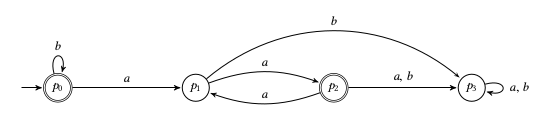
\includegraphics[width=1\linewidth]{Assets/ASK_uebung/u02-01.png}
\end{center}
\textit{(b) Sei $\sum = \{a, b, c\}$. Geben Sie einen DFA an, der die Sprache $L = \{w\in\sum^*\vert |w|_a \leq 1 \text{ und } |w|_b = 0\}$ akzeptiert. Dabei steht für $x\in\sum, w\in\sum^*$ der Ausdruck $|w|_x$ für die Anzahl der x in w.}

%##########################################
\subsection{Aufgabe 6}
\textit{Gegeben seien die folgenden DFAs $M_1$ und $M_2$.}
\begin{center}
    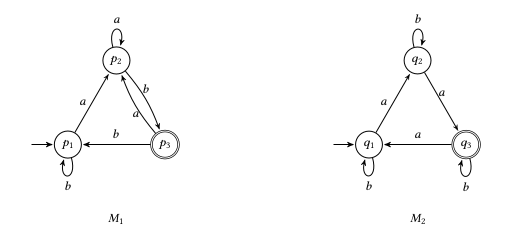
\includegraphics[width=1\linewidth]{Assets/ASK_uebung/u02-02.png}
\end{center}
\textit{Konstruieren Sie folgende Automaten:
    \begin{itemize}
        \item (a) einen DFA $M_\cap$ mit $L(M_\cap) = L(M_1) \cap L(M_2)$,
        \item (b) einen NFA $M_.$ mit $L(M_.) = L(M_1)*L(M_2)$ und
        \item (c) einen NFA $M_* mit L(M_*) = L(M_1)^*$.
    \end{itemize}
}

%##########################################
\subsection{Aufgabe 7}
\textit{Zeigen Sie die folgenden Aussagen:}

\textit{(a) Für jeden NFA $M = (Z , \sum, S, \delta, E)$ existiert ein NFA $M_0 = (Z_0 , \sum, S_0 , \delta_0 , E_0)$ mit $L(M) = L(M_0)$ und $|E_0|=1$.}

\textit{(b) Für jeden NFA $M=(Z,\sum,S,\delta,E)$ existiert ein NFA $M_0=(Z_ 0,\sum,S_0,\delta_0,E_0)$ mit $L(M)=L(M_0)$, $|S_0|=1$ und $|Z_0|=|Z|+1$.}

%##########################################
\subsection{Aufgabe 8}
\textit{Die Spiegelung eines Wortes $w=a_1a_2...a_n\in\sum^*$ sei $w^R := a_na_{n-1}...a_1$ für $a_i\in\sum$ für alle $1\leq i \leq n$. Die Spiegelung einer Sprache $L$ sei $L^R := \{w^R \vert w\in L\}$. Zeigen Sie, dass die Klasse der regulären Sprachen unter Spiegelung abgeschlossen ist.}

\newpage
%%%%%%%%%%%%%%%%%%%%%%%%%%%%%%%%%%%%%%%%%%%%%%%%%%%%%%%%%%%%%%%%%%%%%%%%%%%%%%%%%%%%%%%%%%%%%%%%%%%%%%%%%%%%%%%%%%%%
\section{Übung 03}
%##########################################
\subsection{Aufgabe 1}
\textit{Betrachten Sie die nachfolgenden Sprachen über dem Alphabet $\sum = \{a, b\}$.
    \begin{itemize}
        \item $L_1 = \{w\in\sum^*\vert\text{der vorletzte Buchstabe von w ist ein a}\}$
        \item $L_1 = \sum^*\backslash \{ aa, ab, aab\}$
        \item $L_3 = \{w\in\sum^*\vert\text{ in w kommt ein Buchstabe zweimal direkt hintereinander vor}\}$
        \item $L_4 = \sum^*\backslash L_3$
    \end{itemize}
    Konstruieren Sie für alle $i\in\{1, 2, 3, 4\}$ jeweils einen regulären Ausdruck $r_i$ mit $L(r_i) = L_i$.
}
$$L_1 = (a+b)^* a (a+b)$$

$$L_2 = (b(a+b)^*)+ab(a+b)(a+b)^*+aaa(a+b)^*+aab(a+b)(a+b)^*+a+\lambda$$
\begin{center}
    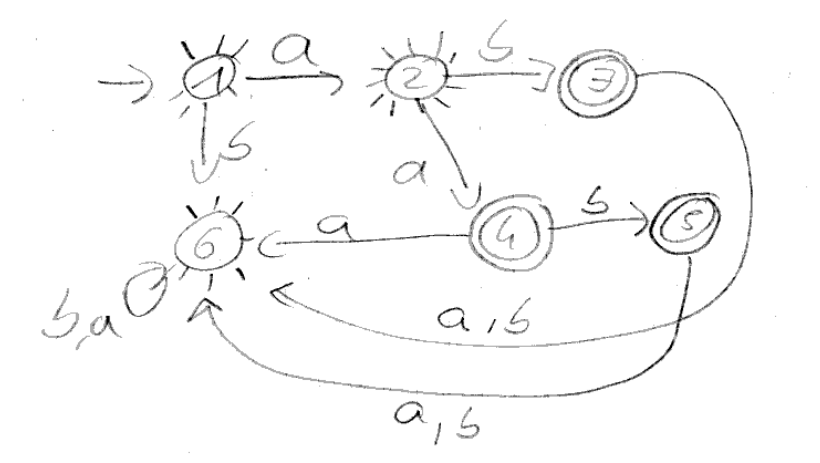
\includegraphics[width=1\linewidth]{Assets/ASK_uebung/u03-01.png}
\end{center}
Idee: Zuerst den Automaten der die aa,ab,aab Sprache akzeptiert aufzeichnen. Dann alle Endzustände (die doppelt umkreisten) zu normalen Zuständen machen und dann die früheren Nicht-Endzustände zu Endzuständen machen (symbolisiert durch die sonnenähnlichen Gebilde um Zustand 1,2,6)

$$L_3 = ((a+b)^*(aa+bb)(a+b)^*(aa+bb)^*(a+b)^*)$$

$$L_4 = (ab)^* + (ba)^*+a+b+\lambda$$


%##########################################
\subsection{Aufgabe 2}
\textit{Zeigen Sie direkt mit dem Pumping-Lemma, dass die Sprache $L=\{a^i b^j \vert i, j\in\mathbb{N}, i > j\}$ nicht regulär ist.}

Behauptung: Die Sprache L ist nicht regulär.
\begin{enumerate}
    \item[0.] Beweis: indirekt. Angenommen L wäre regulär. Nach dem Pumping-Lemma gibt es ein n $\geq$ 1, sodass die folgende Aussage gilt:
          \begin{center}
              Für jedes $x \in L$,  $\mid x \mid \geq n$ gibt es $u,v,w \in\Sigma^*$ mit
              \begin{itemize}
                  \item[i] $x = uvw$
                  \item[ii] $\mid uv \mid\leq n$
                  \item[iii] $\mid v \mid\geq 1$
                  \item[iv] $uv^iw \in L \forall i \geq 0$
              \end{itemize}
          \end{center}
    \item Wir wählen ein Wort $x\in L$. Sei $x = a^nb^j$, wobei n nach Definition der Sprache echt größer $j$ ist.
    \item Nach der Aussage (*) gibt es $u,v,w \in\Sigma^*$, welche die Eigenschaften (i)-(iv) erfüllen.
    \item Sei $x=a^nb^j$ mit $n > j$, wir definieren $j=n-1$.
          Wir wählen $\mid uv \mid < = n$ mit $\mid v\mid\geq k$. Es gilt $v\in\{a\}^+$. Nun sei $i = 0$, damit ist $x=a^{n-k}b^j$, da $\mid v\mid\geq 1$ ist, und da nun $j=n-k$ gilt, ist $n=j$, was allerdings der Bedingung $n>j$ widerspricht. \\
          Wählen wir $\mid v\mid = k$ mit $k\in\mathbb{N}$. so gilt: $uw =a^{(n-k)}b^j$
    \item Dieser Widerspruch von $n = j \neq n > j$ ist ein Widerspruch zu Aussage (iv) des Pumping Lemmas.\\
          Somit ist die Aussage bewiesen, dass die Sprache L nicht regulär sein kann. q.e.d
\end{enumerate}

%##########################################
\subsection{Aufgabe 3}
\textit{Zeigen Sie mit dem Spielschema des Pumping-Lemmas, dass die Sprache $L=\{a^{2^n} | n\in\mathbb{N}\}$ nicht regulär ist.}

\begin{enumerate}
    \item Runde: G wählt eine Zahl $n\geq 1$
    \item Runde: B wählt $x\in L$ mit $\mid x\mid\geq n$. Sei $x = a^{(2^n)}$.
    \item Runde: G wählt $u,v,w$ mit i) $x = u,v,w$ ii) $\mid uv\mid\leq n$ iii) $\mid v\mid\geq 1$
    \item Runde: B wählt $i = 2$ und zeigt, dass $uv^iw \not\in L$ \\
          Sei n beliebig. Wir wählen wie in Runde 2 bereits gesagt $x=a^{2^n}$. Es gilt $x\in L$ und $\mid x\mid\geq n$.\\
          Alle möglichen Stückelungen des Worts sind gemäß der Form: $ u = a^p \quad v = a^q \quad w = a^{2^n}-a^q-a^p$
          mit $p+q \leq n$ und $q\geq 1$.\\
          Wir wählen $i=2$, es gilt $uv^iw = a^{{2^n}+q}$. Es gilt $2^n \geq n \rightarrow p+q < 2^n$ und es gilt weiterhin $0 < q < 2^n$.\\
          Dies bedeutet:$$2^n < 2^n+q < 2^n+2^n = 2*2^n = 2^{n+1}$$
          Hieraus folgt, dass $2^n+q$ keine Zweierpotenz ist, dies wiederum verletzt die Eigenschaften der Sprache und somit ist $uv^iw \notin L$ q.e.d
\end{enumerate}

%##########################################
\subsection{Aufgabe 4}
\textit{Beweisen Sie die folgende verschärfte Version des Pumping-Lemmas: Sei $L\in\sum^*$ eine reguläre Sprache. Dann existiert ein $n>0$, so dass für alle $x\in L$ und alle $x_0,x_1,x_2\in\sum^*$ mit $x=x_0x_1x_2$ und $|x_1|\geq n$ Wörter $u, v, w \in\sum^*$ existieren mit (a) $x_1 = uvw$, (b) $|v| \geq 1$ und
    (c) $x_0 uv^i wx_2\in L$ für alle $i\in\mathbb{N}$.}

Sei $L\subseteq\Sigma^*$ eine reguläre Sprache. Dann exisitiert ein $n>0$, sodass für alle $x\in L$ und alle $x_0,x_1,x_2 \in \Sigma^*$ mit $x = x_0x_1x_2$ und $\mid x_1 \mid \geq n$ Wörter $u,v,w\in \Sigma^*$ existieren mit:
\begin{enumerate}
    \item $x_1$ = uvw
    \item $\mid v \mid \geq 1$ und
    \item $x_0uv^iwx_2 \in L$ für alle $i\in\mathbb{N}$.
\end{enumerate}

Beweis: Sei $n=\mid Z\mid$, wobei Z die Zustände des zugehörigen NFAs $M=(Z,\Sigma,S,\delta,E)$ sind. Ist $x_0x_1x_2 \in L$, so gibt es Zustände $m,n,o\in Z$ mit: $$z_0 \xrightarrow{x_0} m \xrightarrow{x_1} n \xrightarrow{x_2} o \in E$$
Die Transition von m nach n kann in $\mid x_1\mid\geq\mid v\mid +1 \geq n$ Schritten, also durch Begehung von so vielen Zuständen geschehen. Nach der Aussage des Schubkastenprinzips ist dies gleichbedeutend damit, dass zwei der Zustände gleich sein müssen. Nun folgt der Beweis analog dem des einfachen Pumping Lemmas.\\
Es gibt also in $x_1$ Zustände $z_0,z_1,…,z_m$ $\in Z$ mit: $z_0\in S$ (von $x_1$), $z_j \in \delta(z_{j-1},a_j)$ für $1\leq j\leq m$, und $z_m\in E$ (von $x_1$).
Setze $u = a_1 … a_j, v = a_{j+1}…a_k, w=a_{k+1}…a_m$.
Dann gilt:
\begin{itemize}
    \item[i] $x_1 = a_1…a_ja_{j+1}…a_ka_{k+1}…a_m = uvw$ und $x=x_0x_1x_2 = x_0a_1…a_ja_{j+1}…a_ka_{k+1}…a_mx_2 = x_0uvwx_2$
    \item[ii] $\mid uv\mid=\mid a_1…a_k = k \leq n$
    \item[iii] $\mid v\mid = k -(j+1)+1 = k-j > 0$, da ($j < k$)
    \item[iv] Sei $i\geq 0$ beliebig. Es gelten:
          Es führt ein Weg von $z_0\in x_0$ zu dem $z_0^1 \in x_1$ und ein Weg von $z_m^1 \in E \quad von \quad x_1$ nach $z_m \quad von \quad x_2$. Modellieren sozusagen die drei Teilwörter als eigenständige NFAs, bei deren die Überführungen auf die Endzustände der einzelnen NFAs auf die Startzustände des nächsten führen. Betrachten wir nun den NFA zu $x_1$, so folgt nun wie im anderen Beweis auch, dass $uv^iw \in L(x_1)$ ist. Und dies in Kombi mit den weiteren Übergängen $=L$ ist.
\end{itemize}

%##########################################
\subsection{Aufgabe 5}
\textit{Sei $\sum=\{a, b\}$. Wir betrachten die Sprache $L=\{w\in\sum^*\vert\quad |w| \text{ ist gerade und } |w| a \geq 1\}$. Bearbeiten Sie folgende Teilaufgaben:}

\textit{(a) Bestimmen Sie die Myhill-Nerode Äquivalenzklassen von L.}

\textit{(b) Geben Sie den Automaten $M_L$ an}

%##########################################
\subsection{Aufgabe 6}
\textit{Geben Sie einen Algorithmus an, der bei Eingabe eines DFAs M die Größe von $L(M)$ (also $|L(M)|$) berechnet (entweder eine natürliche Zahl $n$ oder $\infty$).}

%##########################################
\subsection{Aufgabe 7}
\textit{Sei $\sum$ ein Alphabet. Zeigen Sie, dass für alle regulären Sprachen $K_1,K_2\subseteq\sum^*$ und ihre Vereinigung $L=K_1\cup K_2$ gilt, dass $Index(R_L)\leq Index(R_{K_1})* Index(R_{K_2})$.}

\newpage
%%%%%%%%%%%%%%%%%%%%%%%%%%%%%%%%%%%%%%%%%%%%%%%%%%%%%%%%%%%%%%%%%%%%%%%%%%%%%%%%%%%%%%%%%%%%%%%%%%%%%%%%%%%%%%%%%%%%
\section{Übung 04}
%##########################################
\subsection{Aufgabe 1}
\textit{Seien $u_1, u_2\in\sum$ zwei Wörter und $L\subseteq\sum$ eine Sprache. Ein trennendes Wort für die Myhill-Nerode Äquivalenz-klassen  $[u_1]_L, [u_2]_L$ ist ein Wort $w\in\sum^*$, so dass $u_1 w\in L, u_2w < L$ oder umgekehrt. Bearbeiten Sie die folgenden Teilaufgaben:}
\textit{Wir betrachten die paarweise verschiedenen Myhill-Nerode Äquivalenzklassen $[\epsilon], [a], [c]$ der Sprache $L_a = \{w\in \{a, b, c\}^* | |w|_a \text{ ist gerade oder } |w| c \geq 1\}$. Geben Sie für jedes Paar von unterschiedlichen Äquivalenzklassen ein trennendes Wort an.}

\textit{Wir betrachten die Myhill-Nerode Äquivalenzklassen der Sprache $L_b = \{0^l 10^m 10^{l +m} | l, m \in\mathbb{N}\}$. Geben Sie für $l\in\mathbb{N}, m\not= m'$ ein trennendes Wort für die Äquivalenzklassen $[0^l 10^m ]$ und $[0^l 10^m]$ an.}


%##########################################
\subsection{Aufgabe 2}
\textit{Wenden Sie das in der Vorlesung vorgestellte Verfahren an, um zu entscheiden, ob die beiden dargestellten DFAs $M_1$ und $M_2$ die gleiche Sprache akzeptieren.}

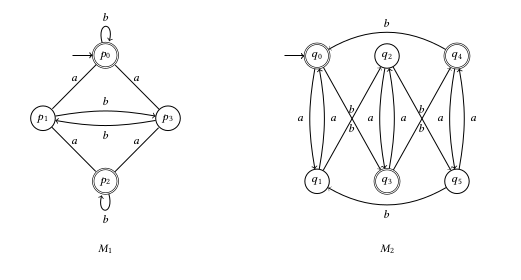
\includegraphics{Assets/ASK_uebung/u04_01.png}


%##########################################
\subsection{Aufgabe 3}
\textit{Wir betrachten das Universalitätsproblem:
    \begin{description}
        \item[Eingabe] NFA $M = (Z , \sum, S, \delta, E)$.
        \item[Frage] Gilt $L(M) = \sum^*$?
    \end{description}
    Geben Sie ein Verfahren an, welches das Universalitätsproblem löst. Begründen Sie Ihre Antwort.}


%##########################################
\subsection{Aufgabe 4}
\textit{In Übung 2 Aufgabe 7 a) haben wir gezeigt, dass es für jeden NFA einen äquivalenten NFA mit genau einem Endzustand gibt. In dieser Aufgabe zeigen wir, dass dies für DFAs nicht der Fall ist. Bearbeiten Sie dazu folgende Teilaufgaben:}

\textit{(a) Geben Sie einen DFA M an, sodass jeder DFA $M_0$ mit $L(M_0) = L(M)$ mindestens zwei akzeptierende Zustände hat.}

\textit{(b) Beweisen Sie, dass Ihr Automat M diese Eigenschaft hat. Hinweis: Es gibt einen Automaten M, der diese Eigenschaft und eine endliche Sprache akzeptiert.}

%##########################################
\subsection{Aufgabe 5}
\textit{In dieser Aufgabe betrachten wir Sprachen für die ein DFA wesentlich mehr Zustände haben muss als ein NFA. Sei $n\in\mathbb{N}$. Wir betrachten die Sprache $K_n= \{w \in \{a, b\}^* | |w| \geq n$ und der n-letzte Buchstabe von w ist ein a}.

\textit{(a) Geben Sie einen NFA mit minimaler Anzahl an Zuständen für $K_n$ an.}

\textit{(b) Bestimmen Sie den Index der Myhill-Nerode Äquivalenz von $K_n$ , $Index(R_{K_n})$. Begründen Sie Ihre Antwort.}

%##########################################
\subsection{Aufgabe 6}
\textit{Sei $\sum = \{a, b\}$. Geben Sie für die folgenden Sprachen jeweils eine kontextfreie Grammatik an.}

\textit{(a) $L_a = \{a_n b_n | n\in\mathbb{N}\}$ }

\textit{(b) $L_b = \{w\in\sum^* | |w|_a = |w|_b \}$ }

\textit{(c) $L_c = \sum^*\backslash \{ww | w\in\sum^*\}$ }


\newpage
%%%%%%%%%%%%%%%%%%%%%%%%%%%%%%%%%%%%%%%%%%%%%%%%%%%%%%%%%%%%%%%%%%%%%%%%%%%%%%%%%%%%%%%%%%%%%%%%%%%%%%%%%%%%%%%%%%%%
\section{Übung 05}
%##########################################
\subsection{Aufgabe 1}
\textit{Entscheiden Sie für jede der folgenden Sprachen, ob sie regulär oder kontextfrei und nicht regulär ist. Geben sie dafür eine rechtslineare Grammatik an oder geben Sie eine kontextfreie Grammatik an und zeigen Sie, dass die Sprache nicht regulär ist.}

\textit{(a) $L_a = \{w\in\{a, b, c\}^* | |w|_a \text{ ist gerade oder } |w|_c \geq 1\}$}

\textit{(b) $L_b = \{uv | u, v \in\{a, b, c\}^* \text{ und } |u|_a > |v|_b \}$ }

\textit{(c) $L_c = \{a^l ba^m ba^n | l = m \text{ oder } l = n\}$ }

\textit{(d) $L_d = \{r \in\{a, b, \lambda,\varnothing, +, ·, * , (, )\}^* | \text{ r ist ein regulärer Ausdruck über }\sum\}$ }

\textit{(e) $L_e = \{r \in L_d | \epsilon\in L(r)\}$ }



%##########################################
\subsection{Aufgabe 2}
\textit{Konstruieren Sie zu zwei kontextfreien Grammatiken $G_1 = (V_1 , \sum, P_1 , S_1 )$ und $G_2 = (V_2 , \sum, P_2 , S_2 )$}

\textit{(a) eine kontextfreie Grammatik $G_{\cup}$ mit $L(G_{\cup}) = L(G_1) \cup L(G_2)$.}

\textit{(b) eine kontextfreie Grammatik $G_{\circ}$ mit $L(G_{\circ}) = L(G_1 ) * L(G_2)$ }.

\textit{(c) eine kontextfreie Grammatik $G_*$ mit $L(G_*) = L(G_1)^*$}

\textit{Hinweis: Sie müssen die Korrektheit Ihrer Konstruktionen nicht beweisen.}


%##########################################
\subsection{Aufgabe 3}
\textit{Wir betrachten die Spiegelung einer Sprache wie in Übung 2, Aufgabe 8. Zeigen Sie, dass die Klasse der kontext-freien Sprachen unter Spiegelung abgeschlossen ist.}



%##########################################
\subsection{Aufgabe 4}
\textit{Betrachten Sie diejenige kontextfreie Grammatik G über $\sum = \{a, b\}$ mit Startvariable $S$, die folgenden Ableitungsbaum $T$ ermöglicht und nicht mehr Produktionen enthält, als für $T$ notwendig sind.}
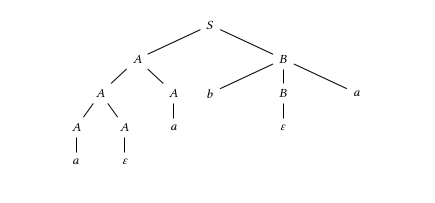
\includegraphics{Assets/ASK_uebung/u06_01.png}
\textit{(a) Geben Sie das Blattwort $\alpha(T)$ von $T$ an und ermitteln Sie weiterhin die Variablen und Produktionen der Grammatik G.}


\textit{(b) Konstruieren Sie die zu $T$ gehörige Links- und Rechtsableitung. Geben Sie eine weitere zu $T$ gehörige Ableitung an, die weder Links- noch Rechtsableitung ist.}


\textit{(c) Geben Sie einen von $T$ verschiedenen S-Ableitungsbaum für das Wort $\alpha(T)$ an. Ist die Grammatik G mehrdeutig?}


\textit{(d) Beschreiben Sie die von G erzeugte Sprache und geben Sie eine eindeutige Grammatik $G_0$ mit $L(G_0) = L(G)$ an.}

%##########################################
\subsection{Aufgabe 5}
\textit{Betrachten Sie die nachstehende Grammatik $G$ mit Startsymbol $S$:\\
    $S\rightarrow BA | a$, $A\rightarrow BS | \epsilon$, $B\rightarrow bBaB | b$}

\textit{(a) Überführen Sie G in eine äquivalente Grammatik $G_0$ in Chomsky-Normalform.}

\textit{(b) Entscheiden Sie mithilfe des CYK-Algorithmus, welche der Wörter $w_1 = bbbaba$ und $w_2 = bbaab$ von Ihrer in (a) berechneten Grammatik erzeugt werden.}

\textit{(c) Geben Sie für diejenigen Wörter aus Aufgabe (b), die von der Grammatik G erzeugt werden, jeweils einen Ableitungsbaum und eine Linksableitung an.}



\newpage
%%%%%%%%%%%%%%%%%%%%%%%%%%%%%%%%%%%%%%%%%%%%%%%%%%%%%%%%%%%%%%%%%%%%%%%%%%%%%%%%%%%%%%%%%%%%%%%%%%%%%%%%%%%%%%%%%%%%
\section{Übung 06}
%##########################################
\subsection{Aufgabe 1}
\textit{Wir betrachten die kontextfreie Grammatik $G$ mit Startvariable $S$ und den folgenden Produktionen:\\
    $S\rightarrow ABC$, $A\rightarrow aA |\epsilon$, $B\rightarrow aDb | D$, $C \rightarrow bC | aC | \epsilon$, $D \rightarrow bDa | ba$\\
    Bearbeiten Sie die folgenden Teilaufgaben:}

\textit{(a) Geben Sie eine kurze Beschreibung von $L(G)$ an.}

\textit{(b) Geben Sie je eine Linksableitung für abab, babaa und abbaab an.}

\textit{(c) Zeigen Sie, dass G eine mehrdeutige Grammatik ist.}

\textit{(d) Zeigen Sie nun, dass $L(G)$ nicht inhärent mehrdeutig ist. Geben Sie also eine eindeutige kontextfreie Grammatik $G_0$ mit $L(G_0) = L(G)$ an. Sie müssen nicht zeigen, dass $G_0$ eindeutig ist.}

%##########################################
\subsection{Aufgabe 2}
\textit{Betrachten Sie die kontextfreie Grammatik G mit Startsymbol S und den nachstehenden Produktionen:\\
    $S\rightarrow Z | (S + S) | (S * S)$, $Z\rightarrow Q | PY$, $Y\rightarrow Q | YY | epsilon$,
    $Q\rightarrow 0 | P$, $P\rightarrow 1$\\
    Bearbeiten Sie folgende Teilaufgaben:}

\textit{(a) Geben Sie eine Ableitung des Wortes $w = (100 + 1)$ in G an und geben Sie eine kurze, aber präzise Beschreibung von $L(G)$ an.}

\textit{(b) Überführen Sie G mit dem Verfahren aus der Vorlesung in eine äquivalente Grammatik $G_0$ in Chomsky-Normalform.}

\textit{(c) Geben Sie eine Ableitung des Wortes w in $G_0$ an.}


%##########################################
\subsection{Aufgabe 3}
\textit{Gegeben sei die kontextfreie Grammatik G in Chomsky-Normalform mit dem Startsymbol S und den Regeln\\
    $S \rightarrow AB | CC$, $A \rightarrow BA | a$, $B \rightarrow AC | b$, $C \rightarrow CC | c$\\
    Überprüfen Sie mithilfe des CYK-Algorithmus, folgende Wörter. Geben Sie für jedes dieser beiden Wörter, welches in $L(G)$ enthalten ist, je eine Ableitung und einen Ableitungsbaum des Wortes an.}

\textit{(a) $aacc \in L(G)$.}

\textit{(b) $bacca \in L(G)$. }



%##########################################
\subsection{Aufgabe 4}
\textit{Wir betrachten den PDA M mit folgender grafischen Darstellung mit Kellerinitialisierungszeichen $\#$:}
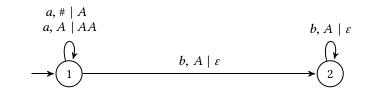
\includegraphics{Assets/ASK_uebung/u06_02.png}

\textit{(a) Gilt $aabb \in L(M)$? Gilt $aabbbb \in L(M)$?}

\textit{(b) Geben Sie eine einfache, aber präzise Beschreibung von $L(M)$ an.}

%##########################################
\subsection{Aufgabe 5}
\textit{Sei $L = \{a^n ba^{2n} | n\in\mathbb{N}\}$.}

\textit{(a) Geben Sie einen PDA $M_1$ an mit $L(M_1) = L$.}

\textit{(b) Geben Sie einen PDA $M_2$ mit genau einem Zustand an mit $L(M_2) = L$.}


%##########################################
\subsection{Aufgabe 6}
\textit{Sei G die kontextfreie Grammatik mit Startvariable A 1 und den folgenden Produktionen. Konstruieren Sie mithilfe des Verfahrens aus der Vorlesung eine Grammatik $G_0$ in Greibach-Normalform mit $L(G_0) = L(G)$.\\
    $A_1\rightarrow 0 | A_2 A_2$, $A_2 \rightarrow 1 | A_1 A_1$}


%##########################################
\subsection{Aufgabe 7}
\textit{Wenden Sie das in der Vorlesung vorgestellte Verfahren an, um zu entscheiden, ob die beiden dargestellten DFAs $M_1$ und $M_2$ die gleiche Sprache akzeptieren.}
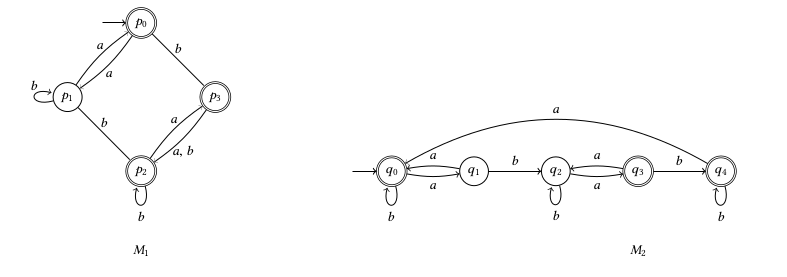
\includegraphics{Assets/ASK_uebung/u06_03.png}


\newpage
%%%%%%%%%%%%%%%%%%%%%%%%%%%%%%%%%%%%%%%%%%%%%%%%%%%%%%%%%%%%%%%%%%%%%%%%%%%%%%%%%%%%%%%%%%%%%%%%%%%%%%%%%%%%%%%%%%%%
\section{Übung 07}
%##########################################
\subsection{Aufgabe 1}
\textit{Die Syntax von Programmiersprachen wird in der Regel in der Erweiterten Backus-Naur-Form 1 (kurz: EBNF) angegeben. Wir wollen in dieser Aufgabe exemplarisch zeigen, dass solche Programmiersprachen kontextfrei sind. Betrachten Sie also die folgende (funktionale) Programmiersprache:
$<Nicht-Null> ::= '1' | '2' | . . . |'9'$\\
$<Zahl> ::= '0' | <Nicht-Null> { '0' | <Nicht-Null> }$\\
$<Variable> ::= 'x' <Zahl>$\\
$<Wert> ::= <Variable> | [ '-' ] <Zahl>$\\
$<Verzweigung> ::= 'if' <Wert> '=' <Wert> 'then' <Programm> [ 'else' <Programm> ]$\\
$<Programm> ::= <Wert> | '(' <Programm> ( '+' | '·' | '-' | ':' ) <Programm> ')' | <Verzweigung>$\\
Geben Sie eine kontextfreie Grammatik an, die alle möglichen Werte von $<Programm>$ erzeugt.}

%##########################################
\subsection{Aufgabe 2}
\textit{Wir betrachten arithmetische Ausdrücke in Präfixnotation über den Konstanten 0,1,2 und mit den Operatoren + (Addition) und * (Multiplikation). Bei der Präfixnotation stehen der Operator vor den Operanden und es gibt keine Klammern. Die Notation ist dennoch eindeutig, so entspricht zum Beispiel $+21$ dem Ausdruck $(2 + 1)$ und $·2++210$ entspricht $(2 · ((2 + 1) + 0))$.}

\textit{(a) Geben Sie eine Regelmenge P an, sodass $G = (\{S, M_0 , M_1 , M_2 \}, \{0, 1, 2, +, *\}, P, S)$ eine kontextfreie Grammatik ist, wobei von S alle arithmetischen Ausdrücke in Präfixnotation erzeugt werden und von $M_i$ alle, die modolu 3 zu i ausgewertet werden.}

\textit{(b) Geben Sie einen Kellerautomaten an, der genau die arithmetischen Ausdrücke in Postfixnotation akzeptiert, die modulo 3 zu 0 ausgewertet werden.}


%##########################################
\subsection{Aufgabe 3}
\textit{Sei $1\leq k \in\mathbb{N}$. Ein k-PDA $M = (Z ,\sum, \Gamma, \delta, z_0 , \#)$ ist ein PDA mit der Eigenschaft, dass der Keller höchstens $k$ Elemente aufnehmen kann. Eine Konfiguration ist also ein Tripel $c\in Z \times\sum^*\times\Gamma^k$ und die Konfigurationsüberführung ist wie folgt definiert: Zunächst wird die Transition wie in den klassischen PDAs ausgeführt und im Falle eines Kellerüberlaufs wird anschließend der Inhalt auf die obersten $k$ Symbole gekürzt. Zeigen Sie, dass die von einem k-PDA M akzeptierte Sprache $L(M)$ regulär ist.}

%##########################################
\subsection{Aufgabe 4}
\textit{Wir betrachten arithmetische Ausdrücke in Postfixnotation über den Konstanten 0,1,2 und mit den Operatoren + (Addition) und * (Multiplikation). Diese Ausdrücke werden von der Grammatik $G = (\{S\}, \{0, 1, 2, +, *\}, P, S)$ erzeugt, wobei P gegeben ist durch: $S \vdash 0 | 1 | 2 | SS+ | SS*$\\
    Hierbei werden zuerst die Operanden und dann der Operator notiert. Zum Beispiel entspricht $12+$ dem Ausdruck $(1+2)$ und $012++2*$ entspricht $((0+(1+2))*2)$. Geben Sie einen Kellerautomaten an, der genau die arithmetischen Ausdrücke in Postfixnotation akzeptiert, die modulo 3 zu 0 ausgewertet werden.
    Hinweis: Es gibt so einen Kellerautomaten mit Kelleralphabet $\Gamma = \{\#, 0, 1, 2\}$.}

%##########################################
\subsection{Aufgabe 5}
\textit{Sei $\sum = \{a, b\}$. Entscheiden Sie für jede der folgenden Sprachen, ob sie kontextfrei oder nicht kontextfrei ist. Beweisen Sie Ihre Aussagen.}

\textit{(a) $L_a = \{a^n ba^n ba^n | n\in\mathbb{N}\}$}

\textit{(b) $L_b = \sum^*\backslash L_a$ }


\newpage
%%%%%%%%%%%%%%%%%%%%%%%%%%%%%%%%%%%%%%%%%%%%%%%%%%%%%%%%%%%%%%%%%%%%%%%%%%%%%%%%%%%%%%%%%%%%%%%%%%%%%%%%%%%%%%%%%%%%
\section{Übung 08}
%##########################################
\subsection{Aufgabe 1}
\textit{Ziel dieser Aufgabe ist es, zu zeigen, dass die Klasse der deterministisch kontextfreien Sprachen nicht unter Vereinigung abgeschlossen ist. Bearbeiten Sie dazu folgende Teilaufgaben:}

\textit{(a) Zeigen Sie, dass die Sprache $\{a^k b^l c^m | k, l, m \in\mathbb{N}, k \not= l \}$ deterministisch kontextfrei ist.}

\textit{(b) Folgern Sie aus (a), dass $L = \{a^k b^l c^m | k, l, m\in\mathbb{N}, k \not= l \text{ oder } k\not=m \text{ oder } l\not=m\}$ kontextfrei ist.}

\textit{(c) Angenommen, L wäre deterministisch kontextfrei. Zeigen Sie, dass unter dieser Annahme auch die Sprache $K=\{a^m b^m c^m | m\in\mathbb{N}\}$ kontextfrei wäre. Hinweis: Verwenden Sie Ergebnisse aus Vorlesung 14.}

\textit{(d) Folgern Sie unter Verwendung aus (a) und (c), dass die Klasse der deterministisch kontextfreien Sprachen nicht unter Vereinigung abgeschlossen ist. Hinweis: Die Sprache K ist nicht kontextfrei.}

%##########################################
\subsection{Aufgabe 2}
\textit{Zeigen Sie, dass folgende Sprachen nicht kontextfrei sind:}

\textit{(a) $L_a = \{a^k b^m a^{k*m} | k, m\in\mathbb{N}\}$ }

\textit{(b) $L_b = \{0^p | p \text{ Primzahl}\}$ }

\textit{(c) $L_c = \{s \# t | s, t\in \{ a, b \}^* \text{ und s ist ein Infix von t } \}$ }

%##########################################
\subsection{Aufgabe 3}
\textit{In dieser Aufgabe zeigen wir, dass die Klasse der deterministisch kontextfreien Sprachen nicht unter Konkatenation abgeschlossen ist.}
\textit{(a) Zeigen Sie, dass $L_2 = \{b^i c^j d^k | i \not= j\} \cup \{ab^i c^j d^k | j \not= k\}$ deterministisch kontextfrei ist.}

\textit{(b) Geben Sie eine deterministisch kontextfreie Sprache $L_1$ an so, dass $L_1* L_2$ nicht deterministisch kontextfrei ist.}

\textit{(c) Zeigen Sie, dass $L_1*L_2$ nicht deterministisch kontextfrei ist.}

%##########################################
\subsection{Aufgabe 4}
\textit{Geben Sie einen Algorithmus an, der folgende Funktion berechnet:
    \begin{description}
        \item[Eingabe] kontextfreie Grammatik G
        \item[Ausgabe:] $|L(G)| \in\mathbb{N}\cup\{\infty\}$
    \end{description}
}



\newpage
%%%%%%%%%%%%%%%%%%%%%%%%%%%%%%%%%%%%%%%%%%%%%%%%%%%%%%%%%%%%%%%%%%%%%%%%%%%%%%%%%%%%%%%%%%%%%%%%%%%%%%%%%%%%%%%%%%%%
\section{Übung 09}
%##########################################
\subsection{Aufgabe 1}
\textit{Beweisen Sie das doppelte Pumping-Lemma für reguläre Sprachen, das wie folgt lautet: Wenn L eine reguläre Sprache ist, dann gibt es $n\geq 1$ derart, dass für alle $z\in L$ mit $|z|\geq n$ gilt: Es gibt Wörter $u, v, w, x, y \in\sum^*$ mit
    \begin{itemize}
        \item (i) $z = uvwxy$
        \item (ii) $|uvwx | \leq n$
        \item (iii) $|v|, |x | \geq 1$
        \item (iv) $uv^i wx^j y\in L$ für alle $i, j\in\mathbb{N}$.
    \end{itemize}
    Hinweis: Orientieren Sie sich am Beweis des Pumping-Lemmas für reguläre Sprachen aus der Vorlesung.}


%##########################################
\subsection{Aufgabe 2}
\textit{Wir betrachten das vereinfachte doppelte Pumping-Lemma für kontextfreie Sprachen (welches nicht gilt): Wenn L eine kontextfreie Sprache ist, dann gibt es $n\geq 1$ derart, dass für alle $z\in L$ mit $|z|\geq n$ gilt: Es gibt Wörter $q, r, s, t, u, v, w, x, y \in\sum^*$ mit
    \begin{itemize}
        \item (i) $z = qrstuvwxy$
        \item (ii) $|rt |, |vx | \geq 1$
        \item (iii) $qr^i st^i uv^j wx^j y \in L$ für alle $i, j\in\mathbb{N}$.
    \end{itemize}
}

\textit{(a) Zeigen Sie, dass die Sprache $\{a^n b^n | n\in\mathbb{N}\}$ ein Gegenbeispiel für das Lemma ist.}

\textit{(b) Formulieren Sie ein gültiges doppeltes Pumping-Lemma für kontextfreie Sprachen. Ein Korrektheitsbeweis ist nicht nötig. Hinweis: Orientieren Sie sich für die Formulierung an Ihrem Beweis aus Aufgabe 1 und an dem Beweis für das Pumping-Lemma für kontextfreie Sprachen aus der Vorlesung.}


%##########################################
\subsection{Aufgabe 3}
\textit{Sei $\sum$ ein Alphabet und $K, L \subseteq\sum^*$. Beweisen Sie die folgenden Aussagen:}

\textit{(a) Ist K deterministisch kontextfrei und L regulär, so ist $K\cap L$ deterministisch kontextfrei.}

\textit{(b) Ist L regulär beziehungsweise kontextfrei, so gilt dies auch für den Abschluss von L unter Präfixen, d.h. für die Sprache $\{u\in\sum^*| \exists v\in\sum^*: uv \in L\}$.}


%##########################################
\subsection{Aufgabe 4}
\textit{Geben Sie einen Algorithmus an, der bei Eingabe eines PDAs M und eines NFAs N entscheidet, ob $L(M)$ Teilmenge von $L(N)$ ist. Anmerkung: Später in der Vorlesung werden wir zeigen, dass es keinen Algorithmus geben kann, der die umgekehrte Teilmengenbeziehung entscheidet.}


%##########################################
\subsection{Aufgabe 5}
\textit{Geben Sie für folgende Funktionen je eine primitiv rekursive Definition und ein Loop-Programm an.}
\textit{(a) $f:\mathbb{N}\rightarrow\mathbb{N}: n\rightarrow n^2$}

\textit{(b) $f:\mathbb{N}\rightarrow\mathbb{N}: n\rightarrow n^n$}


%##########################################
\subsection{Aufgabe 6}
\textit{Zeigen Sie, dass die Funktion $c:\mathbb{N}^2 \rightarrow\mathbb{N}: (m, n) \rightarrow m + \binom{m + n + 1}{2}$ eine Bijektion ist.}


%##########################################
\subsection{Aufgabe 7}
\textit{Geben Sie ein Loop-Programm an, das für zwei gegebene Zahlen $m, n \in\mathbb{N}$ den größten gemeinsamen Teiler berechnet.}




\newpage
%%%%%%%%%%%%%%%%%%%%%%%%%%%%%%%%%%%%%%%%%%%%%%%%%%%%%%%%%%%%%%%%%%%%%%%%%%%%%%%%%%%%%%%%%%%%%%%%%%%%%%%%%%%%%%%%%%%%
\section{Übung 10}
%##########################################
\subsection{Aufgabe 1}
\textit{Geben Sie für folgende Funktionen je eine primitiv rekursive Definition und ein Loop-Programm an:}

\textit{(a) $f:\mathbb{N}\rightarrow\mathbb{N}, n \rightarrow 2^n$}

\textit{(b) $f:\mathbb{N}\rightarrow\mathbb{N}, n \rightarrow n!$ }

%##########################################
\subsection{Aufgabe 2}
\textit{Sei $a(k,n) := ack(k, n) mod 2$, d.h., $a(k, n)$ ist die Parität des Wertes $ack(k, n)$. Zeigen oder widerlegen Sie, dass die Funktion $a$ Loop-berechenbar ist.}


%##########################################
\subsection{Aufgabe 3}
\textit{Sei $(f_k)_{k\in\mathbb{N}}$ eine Folge von Loop-berechenbaren Funktionen $f_k:\mathbb{N}\rightarrow\mathbb{N}$, so dass jedes $f_k$ durch ein Loop-Programm mit k Loop-Schleifen berechnet werden kann, nicht aber durch ein Programm mit $k-1$ Loop-Schleifen. Zeigen oder widerlegen Sie: Die Funktion $g$ mit $g(k, n) = f_k(n)$ ist Loop-berechenbar.}

%##########################################
\subsection{Aufgabe 4}
\textit{Jedes Jahr, kurz vor Heiligabend, startet der Weihnachtsmann auf seinem Keller-Rechner ein Loop-Programm, welches die optimale Route für das Verteilen der Geschenke berechnet. Dieses Jahr geschieht jedoch eine Katastrophe. Schon bei der Eingabe gerät eine Zuckerstange in das Getriebe, wodurch der unendliche Kellerspeicher in sich zusammen fällt. „Oh nein, das war der letzte Rechner mit Kellerspeicher! Woher soll ich denn jetzt wissen, wo ich lang fliegen soll?”, fragt Rudolf. „Ich weiß auch nicht weiter”, sagt der Weihnachtsmann, „Wir haben zwar noch andere Rechner auf denen Loop-Programme laufen, aber der Kellerspeicher ist nötig um den Geschenkstapel auf dem Schlitten zu simulieren.” „Könnten wir nicht den Stack in einem Loop-Programm simulieren?” schlägt ein Wichtel vor. „Das könnte funktionieren. . . ”, sagt der Weihnachtsmann.\\
    Helfen Sie dem Weihnachtsmann, indem Sie zeigen, dass jede Funktion, die durch ein Loop-Programm mit Stack berechnet wird, auch durch ein Loop-Programm ohne Stack berechnet werden kann. Erklärung: Loop-Programme mit Stack verfügen über alle Befehle, die Loop-Programme besitzen. Zusätzlich besitzen sie einen Stack auf den mit dem Befehl $push(x_i)$ der Wert von $x_i$ gelegt werden kann und von dem mit dem Befehl $x_i = pop$ der oberste Wert ausgelesen werden kann, welcher dann gleichzeitig vom Stack entfernt wird. Falls der Stack leer ist gibt $pop$ den Wert $0$ zurück.\\
    Zeigen Sie, dass für jedes Loop-Programm mit Stack, das eine Funktion berechnet, ein Loop-Programm (ohne Stack) existiert, welches die gleiche Funktion berechnet.}

%##########################################
\subsection{Aufgabe 5}
\textit{Welche Funktion berechnet die folgende Turingmaschine M? $M = (\{z_0, z_1, z_2, z_3, z_e\}, \{0, 1\}, \{0, 1,\Box\}, \delta, z_0 , \Box, \{z_e\})$
\begin{tabular}{c|ccc}
        $\delta$ & 0              & 1              & $\Box$            \\\hline
        $z_0$    & $(z_0 , 0, R)$ & $(z_1 , 1, R)$ & $(z_3 , 0, L)$    \\
        $z_1$    & $(z_1 , 0, R)$ & $(z_1 , 1, R)$ & $(z_2 , \Box, L)$ \\
        $z_2$    & $(z_2 , 1, L)$ & $(z_3 , 0, L)$ & $(z_e , 0, N)$   \\
        $z_3$    & $(z_3 , 0, L)$ & $(z_3 , 1, L)$ & $(z_e , \Box, R)$ \\
        $z_e$    & $(z_e , 0, N)$ & $(z_e , 1, N)$ & $(z_e ,\Box, N)$
    \end{tabular}
}

%##########################################
\subsection{Aufgabe 6}
\textit{Geben Sie formal je eine Turingmaschine über dem Alphabet $\sum = \{0, 1\}$ an, die als Eingabe ein Wort $w\in\sum^+$ erhält und}

\textit{(a) den Wert $\lceil w/2 \rceil$ berechnet, wobei $w$ als Binärzahl mit dem höchstwertigsten Bit links betrachtet wird.}

\textit{(b) 1 ausgibt, falls $w$ ein Palindrom ist, und 0 sonst.}

%##########################################
\subsection{Aufgabe 7}
\textit{Geben Sie für jede der folgenden Sprachen je einen PDA an, der die Sprache akzeptiert.}
\textit{(a) $L_1 = \{a^n b^{3n} | n\in\mathbb{N}\}$}

\textit{(b) $L_2 = \{a^n b^m | n \leq m \leq 2n\}$ }

\textit{(c) $L_3 = \{w\in\{a, b\}^* | 2*|w|_a = 3*|w|_b\}$ }

\newpage
%%%%%%%%%%%%%%%%%%%%%%%%%%%%%%%%%%%%%%%%%%%%%%%%%%%%%%%%%%%%%%%%%%%%%%%%%%%%%%%%%%%%%%%%%%%%%%%%%%%%%%%%%%%%%%%%%%%%
\section{Übung 11}
%##########################################
\subsection{Aufgabe 1}
\textit{}

%##########################################
\subsection{Aufgabe 2}
\textit{}


%##########################################
\subsection{Aufgabe 3}
\textit{}




\newpage
%%%%%%%%%%%%%%%%%%%%%%%%%%%%%%%%%%%%%%%%%%%%%%%%%%%%%%%%%%%%%%%%%%%%%%%%%%%%%%%%%%%%%%%%%%%%%%%%%%%%%%%%%%%%%%%%%%%%
\section{Übung 12}
%##########################################
\subsection{Aufgabe 1}
\textit{}

%##########################################
\subsection{Aufgabe 2}
\textit{}


%##########################################
\subsection{Aufgabe 3}
\textit{}




\newpage
%%%%%%%%%%%%%%%%%%%%%%%%%%%%%%%%%%%%%%%%%%%%%%%%%%%%%%%%%%%%%%%%%%%%%%%%%%%%%%%%%%%%%%%%%%%%%%%%%%%%%%%%%%%%%%%%%%%%
\section{Übung 13}
%##########################################
\subsection{Aufgabe 1}
\textit{}

%##########################################
\subsection{Aufgabe 2}
\textit{}


%##########################################
\subsection{Aufgabe 3}
\textit{}




\newpage
%%%%%%%%%%%%%%%%%%%%%%%%%%%%%%%%%%%%%%%%%%%%%%%%%%%%%%%%%%%%%%%%%%%%%%%%%%%%%%%%%%%%%%%%%%%%%%%%%%%%%%%%%%%%%%%%%%%%
\section{Übung 14}
%##########################################
\subsection{Aufgabe 1}
\textit{}

%##########################################
\subsection{Aufgabe 2}
\textit{}


%##########################################
\subsection{Aufgabe 3}
\textit{}




\newpage
%%%%%%%%%%%%%%%%%%%%%%%%%%%%%%%%%%%%%%%%%%%%%%%%%%%%%%%%%%%%%%%%%%%%%%%%%%%%%%%%%%%%%%%%%%%%%%%%%%%%%%%%%%%%%%%%%%%%
\section{Zusätzliche Aufgaben}

\end{document}